\documentclass[notes,11pt, aspectratio=169]{beamer}

\usepackage{pgfpages}
\setbeameroption{hide notes} % Only slide

\usepackage{array}
\usepackage{tikz}
\usepackage{verbatim}
\setbeamertemplate{note page}{\pagecolor{gray!5}\insertnote}
\usetikzlibrary{positioning}
\usetikzlibrary{snakes}
\usetikzlibrary{calc}
\usetikzlibrary{arrows}
\usetikzlibrary{decorations.markings}
\usetikzlibrary{shapes.misc}
\usetikzlibrary{matrix,shapes,arrows,fit,tikzmark}
\usepackage{amsmath}
\usepackage{mathpazo}
\usepackage{hyperref}
\usepackage{lipsum}
\usepackage{multimedia}
\usepackage{graphicx}
\usepackage{multirow}
\usepackage{dcolumn}
\usepackage{bbm}
\newcolumntype{d}[0]{D{.}{.}{5}}

\usepackage{changepage}
\usepackage{appendixnumberbeamer}
\newcommand{\beginbackup}{
   \newcounter{framenumbervorappendix}
   \setcounter{framenumbervorappendix}{\value{framenumber}}
   \setbeamertemplate{footline}
   {
     \leavevmode%
     \hline
     box{%
       \begin{beamercolorbox}[wd=\paperwidth,ht=2.25ex,dp=1ex,right]{footlinecolor}%
       \end{beamercolorbox}}%
     \vskip0pt%
   }
 }
\newcommand{\backupend}{
   \addtocounter{framenumbervorappendix}{-\value{framenumber}}
   \addtocounter{framenumber}{\value{framenumbervorappendix}}
}

\usepackage[space]{grffile}
\usepackage{booktabs}

% Colors
\definecolor{blue}{RGB}{0,114,178}
\definecolor{red}{RGB}{213,94,0}
\definecolor{yellow}{RGB}{240,228,66}
\definecolor{green}{RGB}{0,158,115}
\definecolor{solutionbg}{RGB}{240,248,240}
\definecolor{solutionframe}{RGB}{0,158,115}

% Solution box environment for worked answers
\usepackage{tcolorbox}
\newtcolorbox{solutionbox}[1][]{
  enhanced,
  colback=solutionbg,
  colframe=solutionframe,
  boxrule=0pt,
  leftrule=3pt,
  arc=0pt,
  left=8pt,
  right=8pt,
  top=6pt,
  bottom=6pt,
  fonttitle=\bfseries,
  title={#1},
  attach boxed title to top left={yshift=-2mm, xshift=5mm},
  boxed title style={colback=solutionframe, colframe=solutionframe, size=small, arc=2pt}
}

\hypersetup{
  colorlinks=false,
  linkbordercolor = {white},
  linkcolor = {blue}
}

\definecolor{MyBackground}{RGB}{255,253,218}

\newenvironment{transitionframe}{
  \setbeamercolor{background canvas}{bg=white}
  \begin{frame}}{
    \end{frame}
}

\setbeamercolor{frametitle}{fg=blue}
\setbeamercolor{title}{fg=black}
\setbeamertemplate{footline}[frame number]
\setbeamertemplate{navigation symbols}{}
\setbeamertemplate{itemize items}{-}
\setbeamercolor{itemize item}{fg=blue}
\setbeamercolor{itemize subitem}{fg=blue}
\setbeamercolor{enumerate item}{fg=blue}
\setbeamercolor{enumerate subitem}{fg=blue}
\setbeamercolor{button}{bg=MyBackground,fg=blue,}

\setbeamercolor{section in toc}{fg=blue}
\setbeamercolor{subsection in toc}{fg=red}
\setbeamersize{text margin left=1em,text margin right=1em}

\newenvironment{wideitemize}{\itemize\addtolength{\itemsep}{10pt}}{\enditemize}
\newenvironment{wideenumerate}{\enumerate\addtolength{\itemsep}{10pt}}{\endenumerate}

%%% TIKZ STUFF
\tikzset{
        every picture/.style={remember picture,baseline},
        every node/.style={anchor=base,align=center,outer sep=1.5pt},
        every path/.style={thick},
        }
\newcommand\marktopleft[1]{%
    \tikz[overlay,remember picture]
        \node (marker-#1-a) at (-.3em,.3em) {};%
}
\newcommand\markbottomright[2]{%
    \tikz[overlay,remember picture]
        \node (marker-#1-b) at (0em,0em) {};%
}
\tikzstyle{every picture}+=[remember picture]
\tikzstyle{mybox} =[draw=black, very thick, rectangle, inner sep=10pt, inner ysep=20pt]
\tikzstyle{fancytitle} =[draw=black,fill=red, text=white]
%%%% END TIKZ STUFF

\title[]{\textcolor{blue}{ECN 594: Introduction and Foundations}}
\author[PGP]{}
\institute[FRBNY]{\small{\begin{tabular}{c c c}
Nicholas Vreugdenhil \\
\end{tabular}}}
\date{\today}

\begin{document}

% Title Slide
\begin{frame}
\maketitle
  \centering
\end{frame}

\begin{frame}{Plan}
  \begin{wideenumerate}
    \item \textbf{Introduction and Pricing}
    \item Utility Models and Demand
  \end{wideenumerate}
\end{frame}

%%%%%%%%%%%%%%%%%%%%%%%%%%%%%%%%%%%%%%%%%%%%%%%%%%%%%%%%%%%%%
% INTRODUCTION AND PRICING
%%%%%%%%%%%%%%%%%%%%%%%%%%%%%%%%%%%%%%%%%%%%%%%%%%%%%%%%%%%%%

\begin{frame}{Your economics education so far}
	\begin{wideitemize}
		\item So far in your economics courses you have studied (at least) two forms of competition: \textbf{perfect competition} and \textbf{monopoly}.
		\item We can think of these two forms of competition as polar opposites.
		\item \textbf{Perfect competition} (supply and demand)
		\begin{wideitemize}
			\vspace{5pt}
			\item Many tiny `atomistic' firms
			\item Total surplus is maximized and so the market is `efficient'
		\end{wideitemize}
			\item \textbf{Monopoly}
		\begin{wideitemize}
			\vspace{5pt}
			\item One single firm
			\item Monopoly sets price `too high'; the market is inefficient
		\end{wideitemize}
	\end{wideitemize}
\end{frame}

\begin{frame}{Most real-world markets do not fit neatly into these two categories}
	\begin{wideitemize}
		\item Some examples in this course:
		\begin{wideenumerate}
		\vspace{5pt}
		\item Firms set different prices for the same good (airline tickets, student discounts)
		\item Only a few big firms in the market (health insurance, tech)
		\item Firms collude to raise prices (OPEC, cartels)
		\item Firms merge with other firms (subject to \textbf{antitrust} laws)
		\end{wideenumerate}
	\end{wideitemize}
\end{frame}

\begin{frame}{What is industrial organization (IO)?}
\begin{wideitemize}
	\item \textbf{IO is the study of firm and consumer behavior in markets between (and including) the polar opposites of perfect competition and monopoly.}
	\item Why is this useful?
	\begin{wideenumerate}
		\vspace{11pt}
		\item \underline{Designing regulation/antitrust policy}:
				\vspace{5pt}
				\begin{wideitemize}
					\item When do markets fail? How should we regulate?
				\end{wideitemize}
		\item \underline{Firm strategy}:
				\vspace{5pt}
				\begin{wideitemize}
					\item How to set prices? Design marketplaces?
				\end{wideitemize}
	\end{wideenumerate}
\end{wideitemize}
\end{frame}

\begin{frame}{IO is central to many policy debates right now}
	\begin{wideitemize}
		\item Should we break up Google, Amazon, Meta?
		\item Are hospital mergers raising healthcare costs?
		\item Can algorithms learn to collude?
		\item How should we regulate AI platforms?
	\end{wideitemize}
	\vspace{11pt}
	These are all IO questions.
\end{frame}

\begin{frame}{This course has two components}
	\begin{wideitemize}
		\item \textbf{Theoretical:} Models of pricing, oligopoly, entry, mergers, vertical relationships
		\item \textbf{Empirical:} Demand estimation, merger simulation
	\end{wideitemize}
	\vspace{11pt}
	\begin{wideitemize}
		\item The empirical content (demand estimation) is typically taught at the PhD level
		\item But it's so useful in practice that we cover it here
		\item You'll estimate demand using Python and the \texttt{pyblp} package
	\end{wideitemize}
\end{frame}

\begin{frame}{Course structure}
	\begin{wideenumerate}
		\item \textbf{Part 1 (Lectures 1-7):} Demand Estimation and Pricing
		\begin{wideitemize}
			\vspace{5pt}
			\item Random utility models, logit demand
			\item Identification, instrumental variables
			\item Estimation with \texttt{pyblp}
			\item Price discrimination
		\end{wideitemize}
		\item \textbf{Part 2 (Lectures 8-14):} Competition and Industry Structure
		\begin{wideitemize}
			\vspace{5pt}
			\item Cournot, Bertrand, Hotelling
			\item Entry, mergers, collusion
			\item Vertical relationships
		\end{wideitemize}
	\end{wideenumerate}
\end{frame}

\begin{frame}{Logistics}
	\begin{wideitemize}
		\item E-mail: \texttt{nvreugde@asu.edu}
		\item Office: CRTVC 455G
		\item Office Hours: See syllabus
	\end{wideitemize}
	\vspace{11pt}
	\begin{wideitemize}
		\item \textbf{Textbook:} Cabral, \textit{Introduction to Industrial Organization} (2nd ed.)
		\item For demand estimation: selected readings (posted on Canvas)
	\end{wideitemize}
\end{frame}

\begin{frame}{Assessment}
	\begin{wideitemize}
		\item \textbf{20\%} Homework 1 (demand estimation, Python)
		\item \textbf{20\%} Homework 2 (competition models, merger simulation)
		\item \textbf{30\%} Midterm (Feb 9)
		\item \textbf{30\%} Final (Mar 4)
	\end{wideitemize}
	\vspace{11pt}
	\begin{wideitemize}
		\item Exams: 80 minutes, calculator + one two-sided cheat sheet allowed
	\end{wideitemize}
\end{frame}

\begin{frame}{Building on your prior courses}
	\begin{wideitemize}
		\item From \textbf{ECN 565} (Alvin Murphy): Discrete choice econometrics
		\begin{wideitemize}
			\vspace{5pt}
			\item You know logit, probit, MLE
			\item We'll apply this to IO problems
		\end{wideitemize}
		\item From \textbf{ECN 532} (Hector Chade): Game theory
		\begin{wideitemize}
			\vspace{5pt}
			\item You know Nash equilibrium, Cournot, Bertrand, repeated games
			\item We'll do quick refreshers and focus on IO applications
		\end{wideitemize}
	\end{wideitemize}
\end{frame}

\begin{frame}{Optimal pricing for a monopolist}
\begin{wideitemize}
	\item Now let's discuss \textbf{optimal pricing for a monopolist}.
	\item The `optimal price' is the \textbf{price which maximizes profit}.
	\item Why is this useful?
	\begin{wideitemize}
		\vspace{11pt}
		\item \underline{Policymakers}: understand how the monopolist is reducing welfare
		\item \underline{Firm strategy}: how should you set prices to maximize profits?
	\end{wideitemize}
	\item (Most of this is review from your previous courses)
\end{wideitemize}
\end{frame}

\begin{frame}{Pricing: MR=MC}
	\begin{wideitemize}
		\item The optimal price for a monopolist occurs when:
		\begin{align*}
		 MR = MC
		 \end{align*}
	 	\item This is a \underline{very} important formula.
		\item \textbf{Algorithm to find optimal price:}
		\begin{wideenumerate}
			\vspace{5pt}
			\item Get MR from the demand curve (use `double the slope' if linear)
			\item Set MR = MC; solve for optimal quantity $q^*$
			\item Plug $q^*$ back into demand curve to get optimal price $p^*$
		\end{wideenumerate}
	\end{wideitemize}
\end{frame}

\begin{frame}{Worked example: Monopoly pricing}
	  \begin{wideitemize}
		\item \textbf{Question:}
		\item Suppose a monopolist faces demand $q=2-\frac{1}{5}p$ and has constant marginal cost of 5. What is the optimal price?
	\end{wideitemize}
	\vspace{20pt}
	\centering
	\textit{Take 2 minutes to solve this.}
\end{frame}

\begin{frame}{Worked example: Monopoly pricing (solution)}
	\begin{solutionbox}[Solution]
		\begin{itemize}
			\item First, invert demand: $p=10-5q$
			\item MR using `double the slope': $MR = 10-10q$
			\item Set MR=MC:
			\begin{align*}
				\underbrace{10-10q}_{MR} = \underbrace{5}_{MC}
			\end{align*}
			\item Solve for optimal quantity: $q^*=0.5$
			\item Plug into demand curve: $p^*=10-5 \times 0.5 = 7.5$
		\end{itemize}
	\end{solutionbox}
\end{frame}

\begin{frame}{Pricing: MR=MC (graph)}
\begin{figure}
	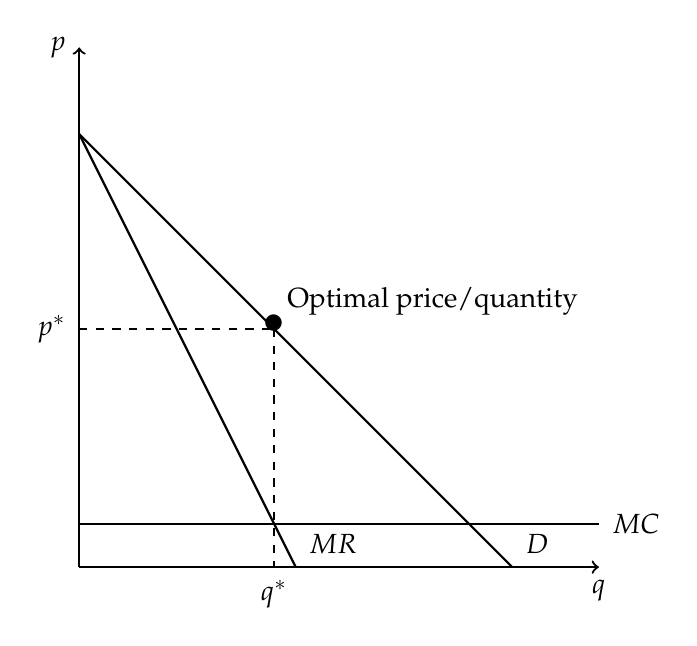
\begin{tikzpicture}[scale=0.55]

		%y axis.....................
		\draw [->] (0,0) to (0,12) node [left] {$p$};

		%x axis......................
		\draw [->] (0,0) to (12,0) node [below] {$q$};

		% D curve...................
		\draw [thick] (0,10)  to  (10,0)  node [above right] {$D$};

		% MR curve....................
		\draw [thick] (0,10) to (5,0);
		\node [above right] at (5,0) {$MR$};

		% MC=S curve...................
		\draw [thick] (0,1)  to  (12,1)  node [right] {$MC$};

		% dashed lines to equilibrium.............
		\draw [dashed] (0,5.5) node [left] {$p^*$} to (4.55,5.5);
		\draw [dashed] (4.5,5.5) to (4.5,0) node [below] {$q^*$};

		% equilibrium points.......................
		\node [black] at (4.5,5.25) {\LARGE \textbullet};

		% labels..............................
		\node [black, above right] at (4.5,5.5) {Optimal price/quantity};

	\end{tikzpicture}
\end{figure}
\end{frame}

\begin{frame}{The Lerner Index}
	\begin{wideitemize}
		\item There is a relationship between the optimal price and demand elasticity.
		\item This is known as the \textbf{Lerner index} (or elasticity rule):
		\begin{align*}
			L = \underbrace{\frac{p-MC}{p}}_{\text{Margin}} = \underbrace{\frac{1}{|\varepsilon|}}_{\text{Inverse elasticity}}
		\end{align*}
		\item The Lerner index measures \textbf{market power}
		\item $L = 0$: perfect competition (price = MC)
		\item $L$ close to 1: high market power
	\end{wideitemize}
\end{frame}

\begin{frame}{Why is the Lerner index useful?}
	\begin{wideitemize}
		\item Suppose you work as an economist in a firm pricing a product.
		\item You know MC. You can estimate the demand elasticity $\varepsilon$.
		\item Then just plug into the elasticity rule:
		\begin{align*}
			p = \frac{MC}{1 + \frac{1}{\varepsilon}}
		\end{align*}
		\item This is exactly what we'll do in Part 1 of this course:
		\begin{wideitemize}
			\vspace{5pt}
			\item Estimate demand $\rightarrow$ get elasticities $\rightarrow$ compute optimal prices
		\end{wideitemize}
	\end{wideitemize}
\end{frame}

\begin{frame}{Welfare costs of monopoly pricing}
	\begin{columns}
		\begin{column}{0.5\textwidth}
			\begin{figure}
				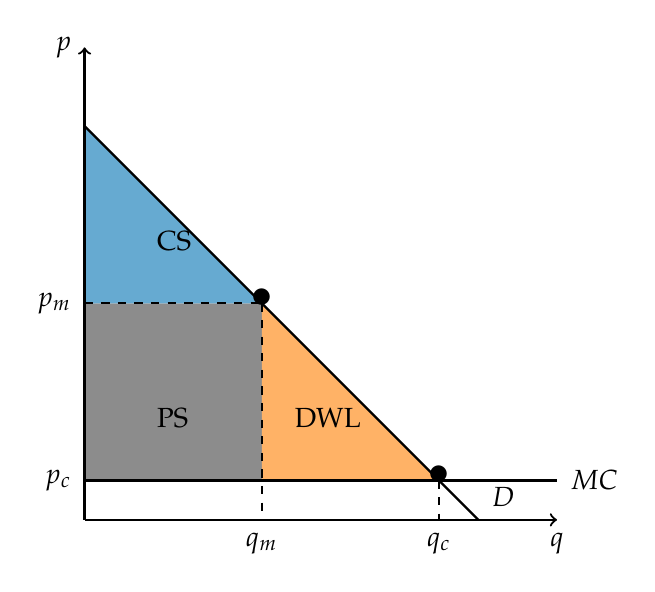
\begin{tikzpicture}[scale=0.5]
					\fill [darkgray!60] (0,1) -- (0,5.5) -- (4.5,5.5) -- (5.5,1) -- cycle;
					\fill [blue!60] (0,5.5) -- (4.5,5.5) -- (0,10) -- cycle;
					\fill [orange!60] (4.5,1) -- (4.5,5.5) -- (9,1) -- cycle;

					%y axis.....................
					\draw [->] (0,0) to (0,12) node [left] {$p$};

					%x axis......................
					\draw [->] (0,0) to (12,0) node [below] {$q$};

					% D curve...................
					\draw [thick] (0,10)  to  (10,0)  node [above right] {$D$};

					% MC=S curve...................
					\draw [thick] (0,1)  to  (12,1)  node [right] {$MC$};

					% dashed lines to equilibrium.............
					\draw [dashed] (0,5.5) node [left] {$p_m$} to (4.55,5.5);
					\draw [dashed] (4.5,5.5) to (4.5,0) node [below] {$q_m$};

					% dashed lines to new equilibrium.........
					\draw [dashed] (0,1) node [left] {$p_{c}$} to (9,1);
					\draw [dashed] (9,1) to (9,0) node [below] {$q_{c}$};

					% equilibrium points.......................
					\node [black] at (4.5,5.25) {\LARGE \textbullet};
					\node [black] at (9,0.75) {\LARGE \textbullet};

					% labels..............................
					\node [above right] at (1.5,6.5) {CS};
					\node [above right] at (5,2) {DWL};
					\node [above right] at (1.5,2) {PS};
				\end{tikzpicture}
			\end{figure}
		\end{column}
		\begin{column}{0.5\textwidth}
			\begin{wideitemize}
				\item Competitive outcome: $p_c$, $q_c$
				\item Monopoly outcome: $p_m$, $q_m$
				\item Monopoly sets price `too high' and quantity `too low'
				\item This causes \textbf{deadweight loss} (DWL)
				\item Monopoly is a \textbf{market failure}
			\end{wideitemize}
		\end{column}
	\end{columns}
\end{frame}

\begin{frame}{Regulating monopolies}
	\begin{wideitemize}
		\item How can we correct the market failure of monopoly?
		\item \textbf{Option 1:} Break up the monopoly (antitrust)
		\begin{wideitemize}
			\vspace{5pt}
			\item Standard Oil (1911), AT\&T (1984)
			\item Current debates: Google, Meta, Amazon
		\end{wideitemize}
		\item Sometimes breaking up isn't possible (natural monopolies)
		\begin{wideitemize}
			\vspace{5pt}
			\item Power plants, bridges, water utilities
			\item High fixed costs make one firm efficient
		\end{wideitemize}
		\item How should we regulate these natural monopolies?
	\end{wideitemize}
\end{frame}

\begin{frame}{Marginal cost pricing}
	\begin{wideitemize}
		\item \textbf{Idea:} Force the monopolist to set $p=MC$
		\begin{wideitemize}
			\vspace{5pt}
			\item This is the competitive price; no deadweight loss
		\end{wideitemize}
		\item \textbf{Problem:} Suppose cost is $C(q) = F + cq$ (fixed cost + marginal cost)
		\item If $p=MC=c$, then profit is:
		\begin{align*}
			\pi = pq - F - cq = cq - F - cq = -F < 0
		\end{align*}
		\item Firm makes \textbf{negative} profit and would shut down!
		\item Solution: government \textbf{subsidy} of $F$
	\end{wideitemize}
\end{frame}

\begin{frame}{Average cost pricing}
	\begin{wideitemize}
		\item \textbf{Alternative:} Force the monopolist to set $p=AC$
		\item This is the price where the monopolist makes zero profit:
		\begin{wideitemize}
			\vspace{5pt}
			\item If $\pi = 0$ then $TR = TC$
			\item So $pq = TC$, which means $p = TC/q = AC$
		\end{wideitemize}
		\item The monopolist can only exercise market power to cover fixed costs
		\item No government subsidy needed
		\item Commonly used for utilities (``rate of return regulation'')
	\end{wideitemize}
\end{frame}

\begin{frame}{Average cost pricing (graph)}
	\begin{figure}
		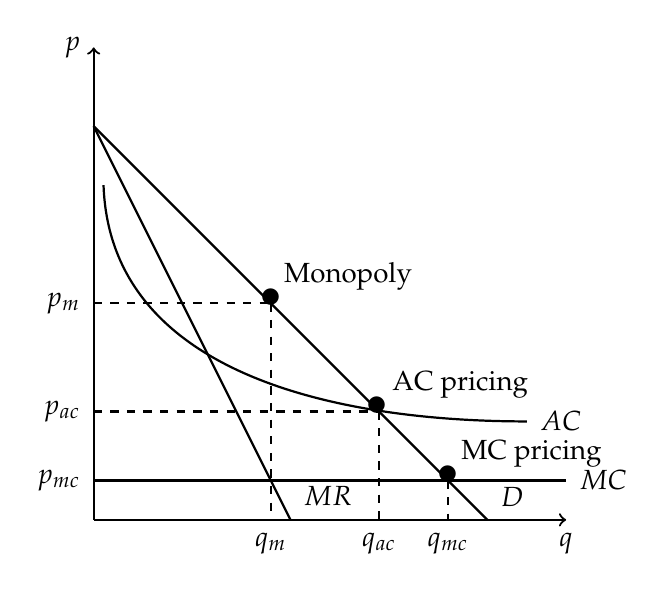
\begin{tikzpicture}[scale=0.5]

			%y axis.....................
			\draw [->] (0,0) to (0,12) node [left] {$p$};

			%x axis......................
			\draw [->] (0,0) to (12,0) node [below] {$q$};

			% D curve...................
			\draw [thick] (0,10)  to  (10,0)  node [above right] {$D$};

			% MR curve....................
			\draw [thick] (0,10) to (5,0);
			\node [above right] at (5,0) {$MR$};

			% MC=S curve...................
			\draw [thick] (0,1)  to  (12,1)  node [right] {$MC$};

			% ATC curve...................
			\draw [thick] (0.25,8.5) to [out=-88,in=180]  (11,2.5) node[right] {$AC$};

			% dashed lines to equilibrium.............
			\draw [dashed] (0,5.5) node [left] {$p_m$} to (4.55,5.5);
			\draw [dashed] (4.5,5.5) to (4.5,0) node [below] {$q_m$};

			% dashed lines to mc pricing.........
			\draw [dashed] (0,1) node [left] {$p_{mc}$} to (9,1);
			\draw [dashed] (9,1) to (9,0) node [below] {$q_{mc}$};

			% dashed lines to ac pricing.........
			\draw [dashed] (0,2.75) node [left] {$p_{ac}$} to (7.25,2.75);
			\draw [dashed] (7.25,2.75) to (7.25,0) node [below] {$q_{ac}$};

			% equilibrium points.......................
			\node [black] at (4.5,5.25) {\LARGE \textbullet};
			\node [black] at (7.2,2.5) {\LARGE \textbullet};
			\node [black] at (9,0.75) {\LARGE \textbullet};

			% labels..............................
			\node [black, above right] at (4.5,5.5) {Monopoly};
			\node [black, above right] at (7.25,2.75) {AC pricing};
			\node [black, above right] at (9,1) {MC pricing};
		\end{tikzpicture}
	\end{figure}
\end{frame}

\begin{frame}{Price caps}
	\begin{wideitemize}
		\item \textbf{Price cap regulation:} Set a maximum price the firm can charge
		\item Often indexed to inflation (``CPI-X'' regulation)
		\begin{wideitemize}
			\vspace{5pt}
			\item Price can rise with inflation, minus an efficiency factor X
		\end{wideitemize}
		\item Advantage: incentivizes cost reduction
		\begin{wideitemize}
			\vspace{5pt}
			\item Under AC pricing, firm has no incentive to cut costs
			\item Under price caps, cost savings become profit
		\end{wideitemize}
		\item Common in UK utilities, telecoms
	\end{wideitemize}
\end{frame}

%%%%%%%%%%%%%%%%%%%%%%%%%%%%%%%%%%%%%%%%%%%%%%%%%%%%%%%%%%%%%
% UTILITY MODELS AND DEMAND
%%%%%%%%%%%%%%%%%%%%%%%%%%%%%%%%%%%%%%%%%%%%%%%%%%%%%%%%%%%%%

\begin{frame}{Plan}
  \begin{wideenumerate}
    \item Introduction and Pricing
    \item \textbf{Utility Models and Demand}
  \end{wideenumerate}
\end{frame}

\begin{frame}{Why is estimating demand useful?}
	  \begin{wideitemize}
		\item Quantifying market power (think: Lerner index)
		\item Effects of a merger on prices
		\item Value of new goods
		\item Any question about consumer welfare
		\item Numerous other applications: school choice, health insurance, etc.
	\end{wideitemize}
\end{frame}

\begin{frame}{Why is estimating demand useful?}
	\begin{wideitemize}
		\item Recall: Lerner index $L = (p-MC)/p = 1/|\varepsilon|$
		\item To compute market power, we need the \textbf{demand elasticity} $\varepsilon$
		\item How do we get the elasticity?
		\item We need to \textbf{estimate demand}
		\item This is one of the key empirical methods in IO
	\end{wideitemize}
\end{frame}

\begin{frame}{Ordinal vs cardinal utility}
	\begin{wideitemize}
		\item \textbf{Ordinal utility:} only rankings matter, not magnitudes
		\begin{wideitemize}
			\vspace{5pt}
			\item $U(A) > U(B)$ means I prefer A to B
			\item But ``$U(A) = 2 \times U(B)$'' has no meaning
		\end{wideitemize}
		\item This is the standard microeconomics assumption
		\item \textbf{Problem:} We want to measure consumer surplus in \$!
		\begin{wideitemize}
			\vspace{5pt}
			\item ``How much better off are consumers from this policy?''
			\item Need utility to have a meaningful \textit{scale}
		\end{wideitemize}
	\end{wideitemize}
\end{frame}

\begin{frame}{Quasi-linear utility makes utility cardinal}
	\begin{wideitemize}
		\item \textbf{Solution:} Assume quasi-linear utility
		\begin{align*}
			U = u(\text{goods}) + y
		\end{align*}
		where $y$ is income (or ``money left over'')
		\item Take the derivative with respect to income:
		\begin{align*}
			\frac{\partial U}{\partial y} = 1
		\end{align*}
		\item The \textbf{marginal utility of income is constant} (and equals 1)
		\item This means we can measure utility in dollars!
	\end{wideitemize}
\end{frame}

\begin{frame}{Why this matters}
	\begin{wideitemize}
		\item With quasi-linear utility:
		\begin{wideitemize}
			\vspace{5pt}
			\item 1 util = \$1
			\item Consumer surplus has a meaningful interpretation
			\item We can add up utility across consumers
		\end{wideitemize}
		\item This is the standard assumption in IO demand estimation
		\item (In contrast to general equilibrium models where income effects matter)
	\end{wideitemize}
\end{frame}

\begin{frame}{Random utility framework (refresher from ECN 565)}
	\begin{wideitemize}
		\item Consumer $i$ chooses among $J$ products
		\item Utility of consumer $i$ for product $j$:
		\begin{align*}
			u_{ij} = V_{ij} + \varepsilon_{ij}
		\end{align*}
		\item $V_{ij}$: deterministic component (observed by econometrician)
		\item $\varepsilon_{ij}$: random component (taste shock)
	\end{wideitemize}
\end{frame}

\begin{frame}{Random utility framework}
	\begin{wideitemize}
		\item Consumer $i$ chooses product $j$ if:
		\begin{align*}
			u_{ij} > u_{ik} \quad \text{for all } k \neq j
		\end{align*}
		\item Choice probability:
		\begin{align*}
			P(i \text{ chooses } j) = P(u_{ij} > u_{ik} \text{ for all } k)
		\end{align*}
		\item Different assumptions on $\varepsilon_{ij}$ give different models:
		\begin{wideitemize}
			\vspace{5pt}
			\item Type I Extreme Value $\rightarrow$ \textbf{Logit}
			\item Normal $\rightarrow$ \textbf{Probit}
		\end{wideitemize}
		\item You covered this in ECN 565; we'll apply it to IO
	\end{wideitemize}
\end{frame}

\begin{frame}{Discrete choice in IO}
	\begin{wideitemize}
		\item In IO, we typically write:
		\begin{align*}
			u_{ij} = x_j \beta - \alpha p_j + \xi_j + \varepsilon_{ij}
		\end{align*}
		\item $x_j$: observed product characteristics (size, horsepower, etc.)
		\item $p_j$: price
		\item $\xi_j$: unobserved product quality
		\item $\varepsilon_{ij}$: idiosyncratic taste shock
		\item $\alpha > 0$: price coefficient (enters negatively!)
	\end{wideitemize}
\end{frame}

\begin{frame}{What is $\xi_j$?}
	\begin{wideitemize}
		\item $\xi_j$ = unobserved product quality
		\item Examples:
		\begin{wideitemize}
			\vspace{5pt}
			\item Brand equity (``I just like Toyota'')
			\item Advertising effects
			\item Design/style
			\item Reputation
		\end{wideitemize}
		\item Key insight: firms \textit{observe} $\xi_j$ when setting prices!
		\item This creates an endogeneity problem (more on this next lecture)
	\end{wideitemize}
\end{frame}

\begin{frame}{Why isn't income in the utility function?}
	\begin{wideitemize}
		\item You might expect: $u_{ij} = x_j \beta + \alpha (y_i - p_j) + \xi_j + \varepsilon_{ij}$
		\item But we write: $u_{ij} = x_j \beta - \alpha p_j + \xi_j + \varepsilon_{ij}$
		\item \textbf{Why?}
		\item With quasi-linear utility, income enters linearly
		\item When comparing alternatives, income \textit{cancels out}:
		\begin{align*}
			u_{ij} - u_{ik} &= [x_j \beta + \alpha(y_i - p_j) + \xi_j + \varepsilon_{ij}] \\
			&\quad - [x_k \beta + \alpha(y_i - p_k) + \xi_k + \varepsilon_{ik}] \\
			&= (x_j - x_k)\beta - \alpha(p_j - p_k) + (\xi_j - \xi_k) + (\varepsilon_{ij} - \varepsilon_{ik})
		\end{align*}
		\item Only \textit{differences} matter for choice, and $y_i$ drops out
	\end{wideitemize}
\end{frame}

\begin{frame}{The outside option}
	\begin{wideitemize}
		\item Important: Consumers can choose \textbf{not to buy} any product
		\item This is the \textbf{outside option} (product 0)
		\item Utility of outside option:
		\begin{align*}
			u_{i0} = \varepsilon_{i0}
		\end{align*}
		\item We normalize non-idiosyncratic components to 0
		\item All other utilities are \textit{relative} to the outside option
		\item Why this matters:
		\begin{wideitemize}
			\vspace{5pt}
			\item If prices rise, consumers can ``exit'' the market
			\item This affects elasticities and market power
		\end{wideitemize}
	\end{wideitemize}
\end{frame}

\begin{frame}{The dimensionality problem}
	\begin{wideitemize}
		\item Suppose we have $J$ products in the market
		\item What do we need to describe demand fully?
		\item \textbf{Own-price elasticities:} $J$ elasticities
		\item \textbf{Cross-price elasticities:} $J \times (J-1)$ elasticities
		\item Total: $J^2$ elasticities!
		\item For $J = 100$ products: 10,000 elasticities to estimate
	\end{wideitemize}
\end{frame}

\begin{frame}{The dimensionality problem: solution}
	\begin{wideitemize}
		\item \textbf{Key idea:} Products are bundles of characteristics
		\item Consumers have preferences over characteristics, not products
		\begin{align*}
			u_{ij} = x_j \beta - \alpha p_j + \xi_j + \varepsilon_{ij}
		\end{align*}
		\item Instead of $J^2$ elasticities, we estimate:
		\begin{wideitemize}
			\vspace{5pt}
			\item $K$ coefficients on characteristics ($\beta$)
			\item 1 price coefficient ($\alpha$)
		\end{wideitemize}
		\item Cross-price elasticities come out of the model structure
		\item Products with similar characteristics are close substitutes
	\end{wideitemize}
\end{frame}

\begin{frame}{Example: Cars}
	\begin{wideitemize}
		\item Product characteristics $x_j$:
		\begin{wideitemize}
			\vspace{5pt}
			\item Size (length, weight)
			\item Horsepower
			\item Fuel efficiency (MPG)
			\item Air conditioning, etc.
		\end{wideitemize}
		\item A Honda Civic and Toyota Corolla have similar characteristics
		\item $\Rightarrow$ They are close substitutes
		\item A Honda Civic and BMW 7-Series have different characteristics
		\item $\Rightarrow$ They are not close substitutes
		\item This structure comes from the model, not from estimating $J^2$ elasticities
	\end{wideitemize}
\end{frame}

%%%%%%%%%%%%%%%%%%%%%%%%%%%%%%%%%%%%%%%%%%%%%%%%%%%%%%%%%%%%%
% KEY POINTS
%%%%%%%%%%%%%%%%%%%%%%%%%%%%%%%%%%%%%%%%%%%%%%%%%%%%%%%%%%%%%

\begin{frame}{Key Points}
	\vspace{11pt}
	\begin{wideenumerate}
		\item \textbf{IO} studies firm behavior between perfect competition and monopoly
		\item This course has \textbf{theory} (pricing, oligopoly) and \textbf{empirical} (demand estimation) components
		\item \textbf{Monopoly pricing:} $MR = MC$; Lerner index $L = (p-MC)/p = 1/|\varepsilon|$
		\item Monopoly causes \textbf{deadweight loss}; regulation options include MC pricing, AC pricing, price caps
		\item \textbf{Demand estimation} is central to IO: elasticities $\rightarrow$ market power $\rightarrow$ policy
		\item \textbf{Quasi-linear utility} makes consumer surplus measurable in \$
		\item \textbf{Random utility:} $u_{ij} = x_j \beta - \alpha p_j + \xi_j + \varepsilon_{ij}$
		\item \textbf{Characteristics-based models} solve the dimensionality problem
	\end{wideenumerate}
\end{frame}

\begin{frame}{Next time}
	\begin{wideitemize}
		\item \textbf{Lecture 2:} The Logit Model and Identification
		\begin{wideitemize}
			\vspace{5pt}
			\item Logit derivation and elasticity formulas
			\item Why price is endogenous
			\item Instrumental variables
		\end{wideitemize}
	\end{wideitemize}
\end{frame}

\end{document}
